\documentclass[12pt,a4paper,dvipdfmx,titlepage]{jsarticle}
\usepackage[top=25truemm,bottom=25truemm,left=25truemm,right=25truemm]{geometry}
\usepackage{graphicx}
\usepackage{float}
\usepackage{url}
\usepackage{cite}
\bibliographystyle{jplain}

\begin{document}

\title{
    データの可視化 \\
    \large 課題実習レポート
}

\author{1021120 及川 寛太}

\date{2024年1月17日}

\maketitle

\section*{可視化表現}
画像は,以下に示す.
インタラクティブな操作ができるWebページ\footnote{https://bit.ly/4aUdoP3}を用意した.
また,そこでの動きがわかる動画\footnote{https://bit.ly/3HndaSP}を用意した.

\begin{figure}[H]
    \centering
    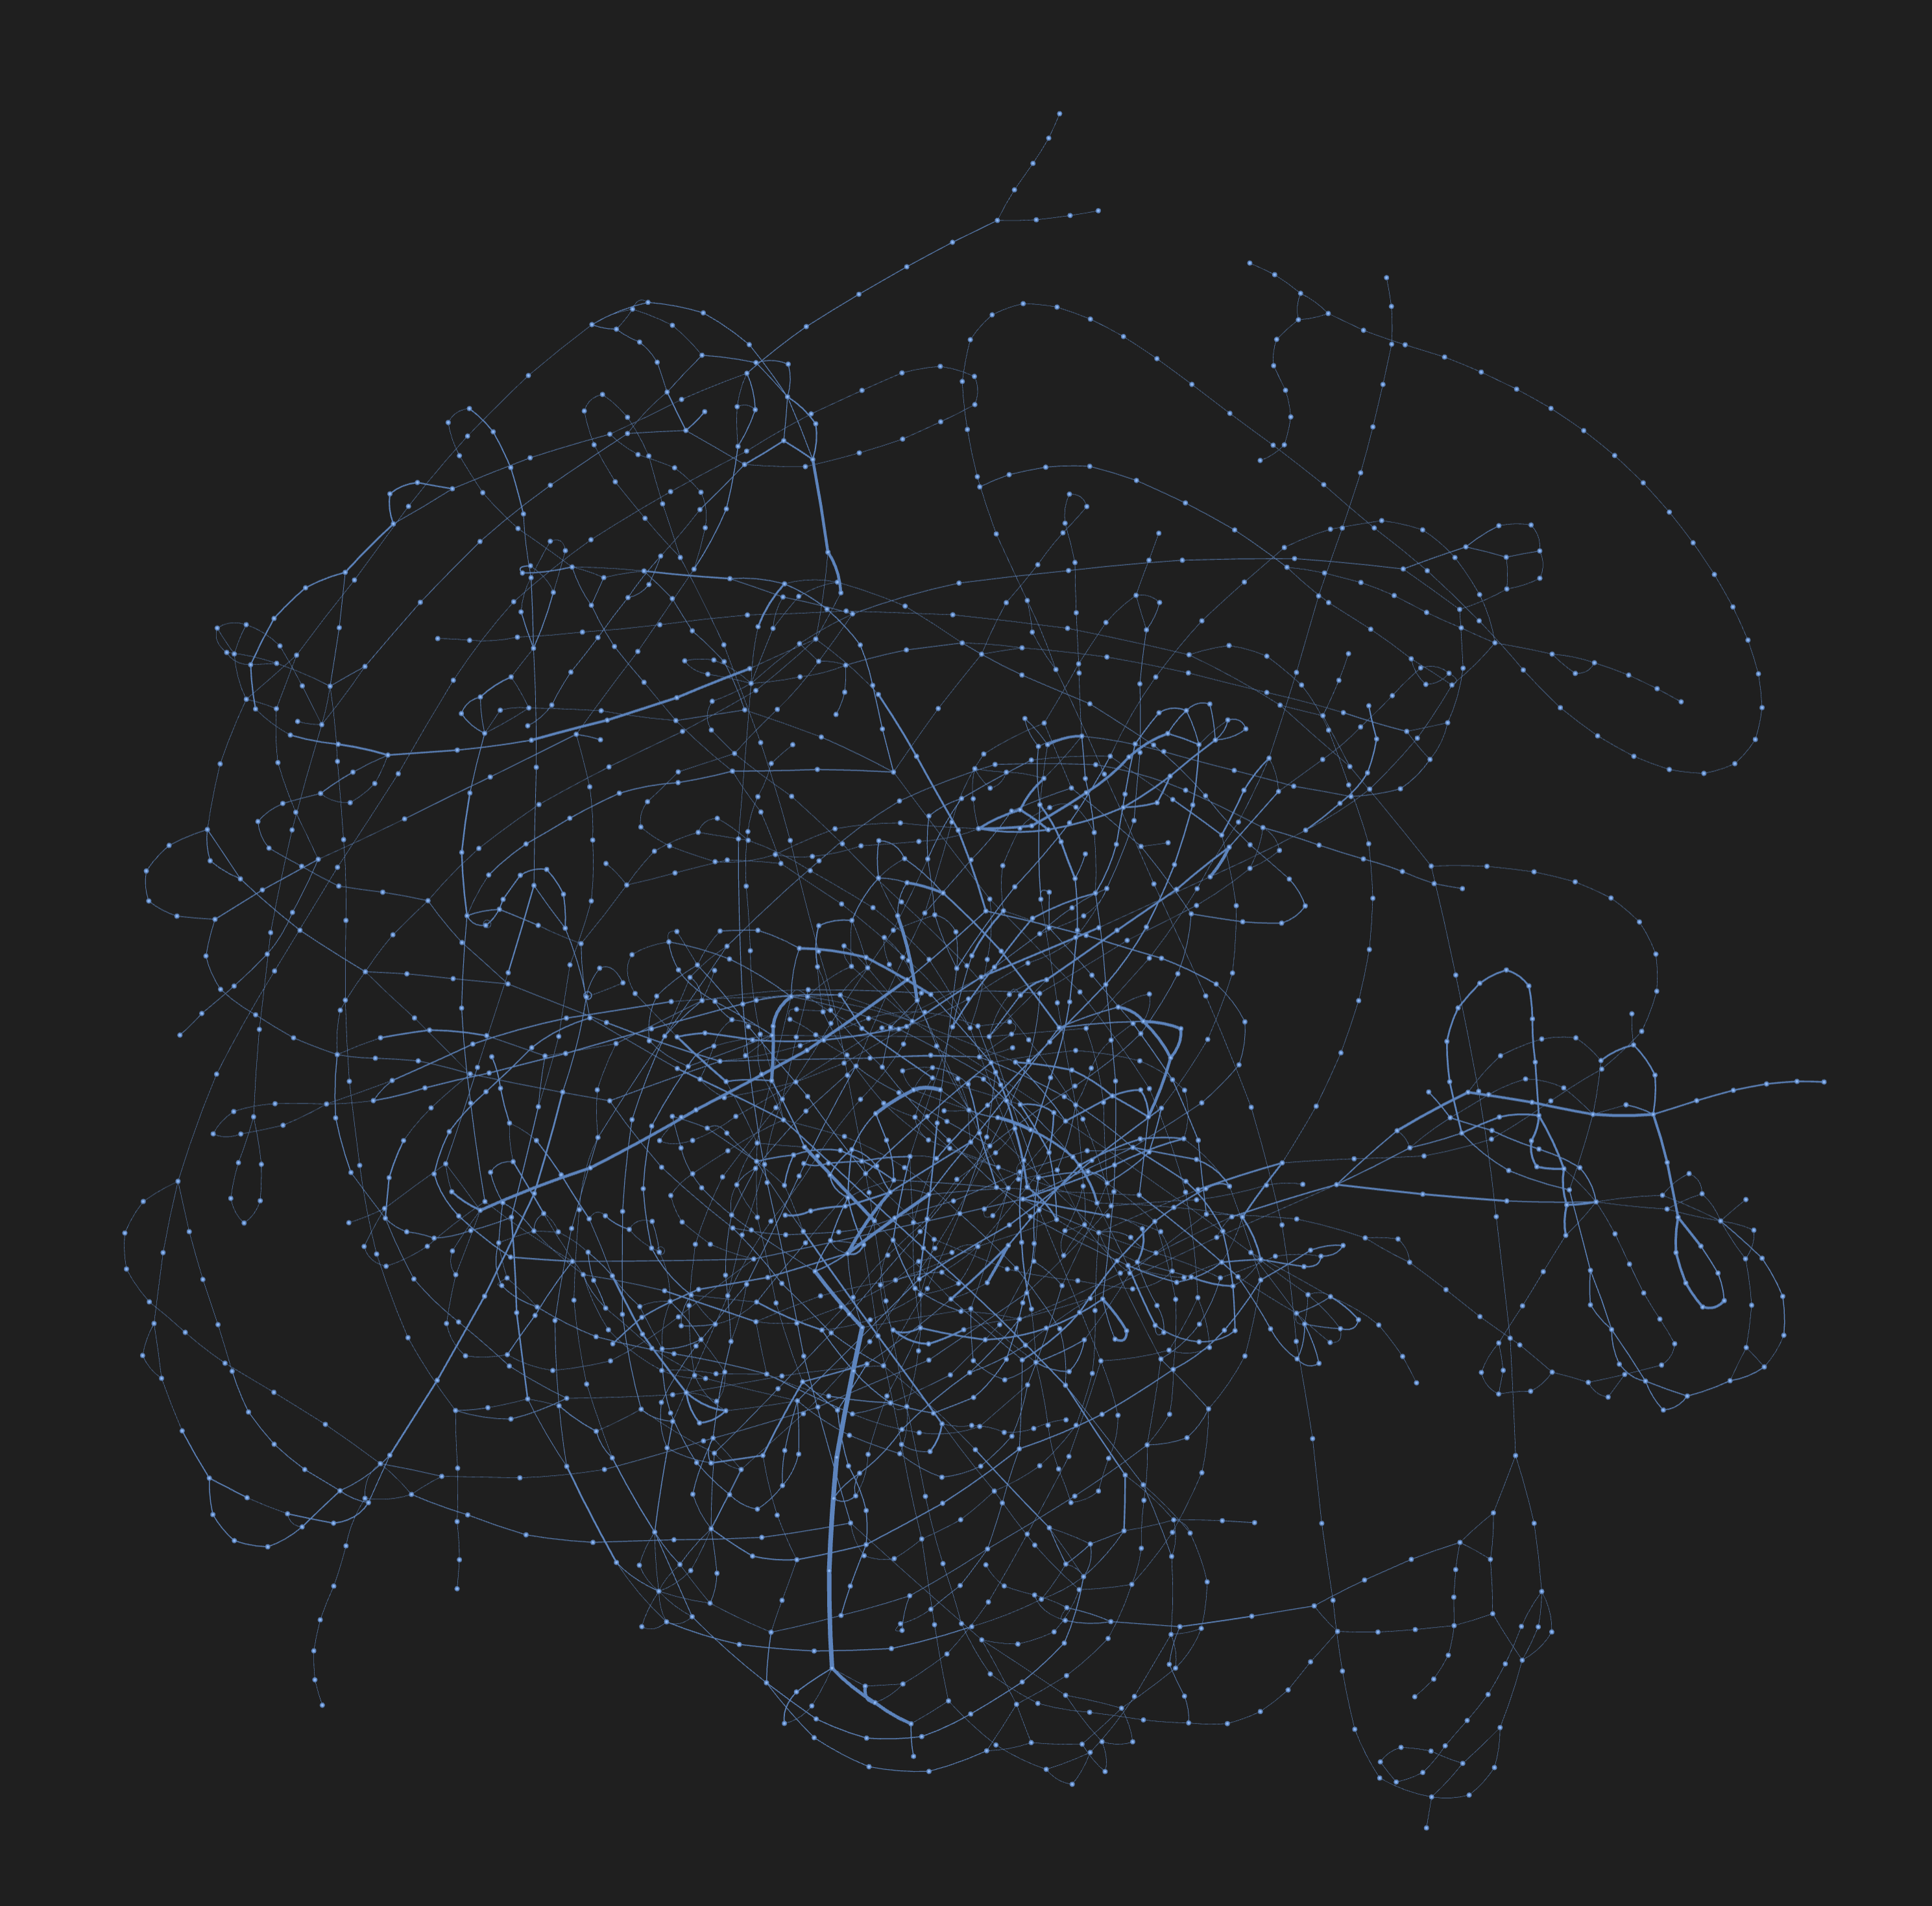
\includegraphics[width=10cm]{./img/fig1.png}
    \caption{可視化表現 ネットワークレイアウト アークグラフ (俯瞰)}
    \label{fig:fig1}
\end{figure}

\begin{figure}[H]
    \centering
    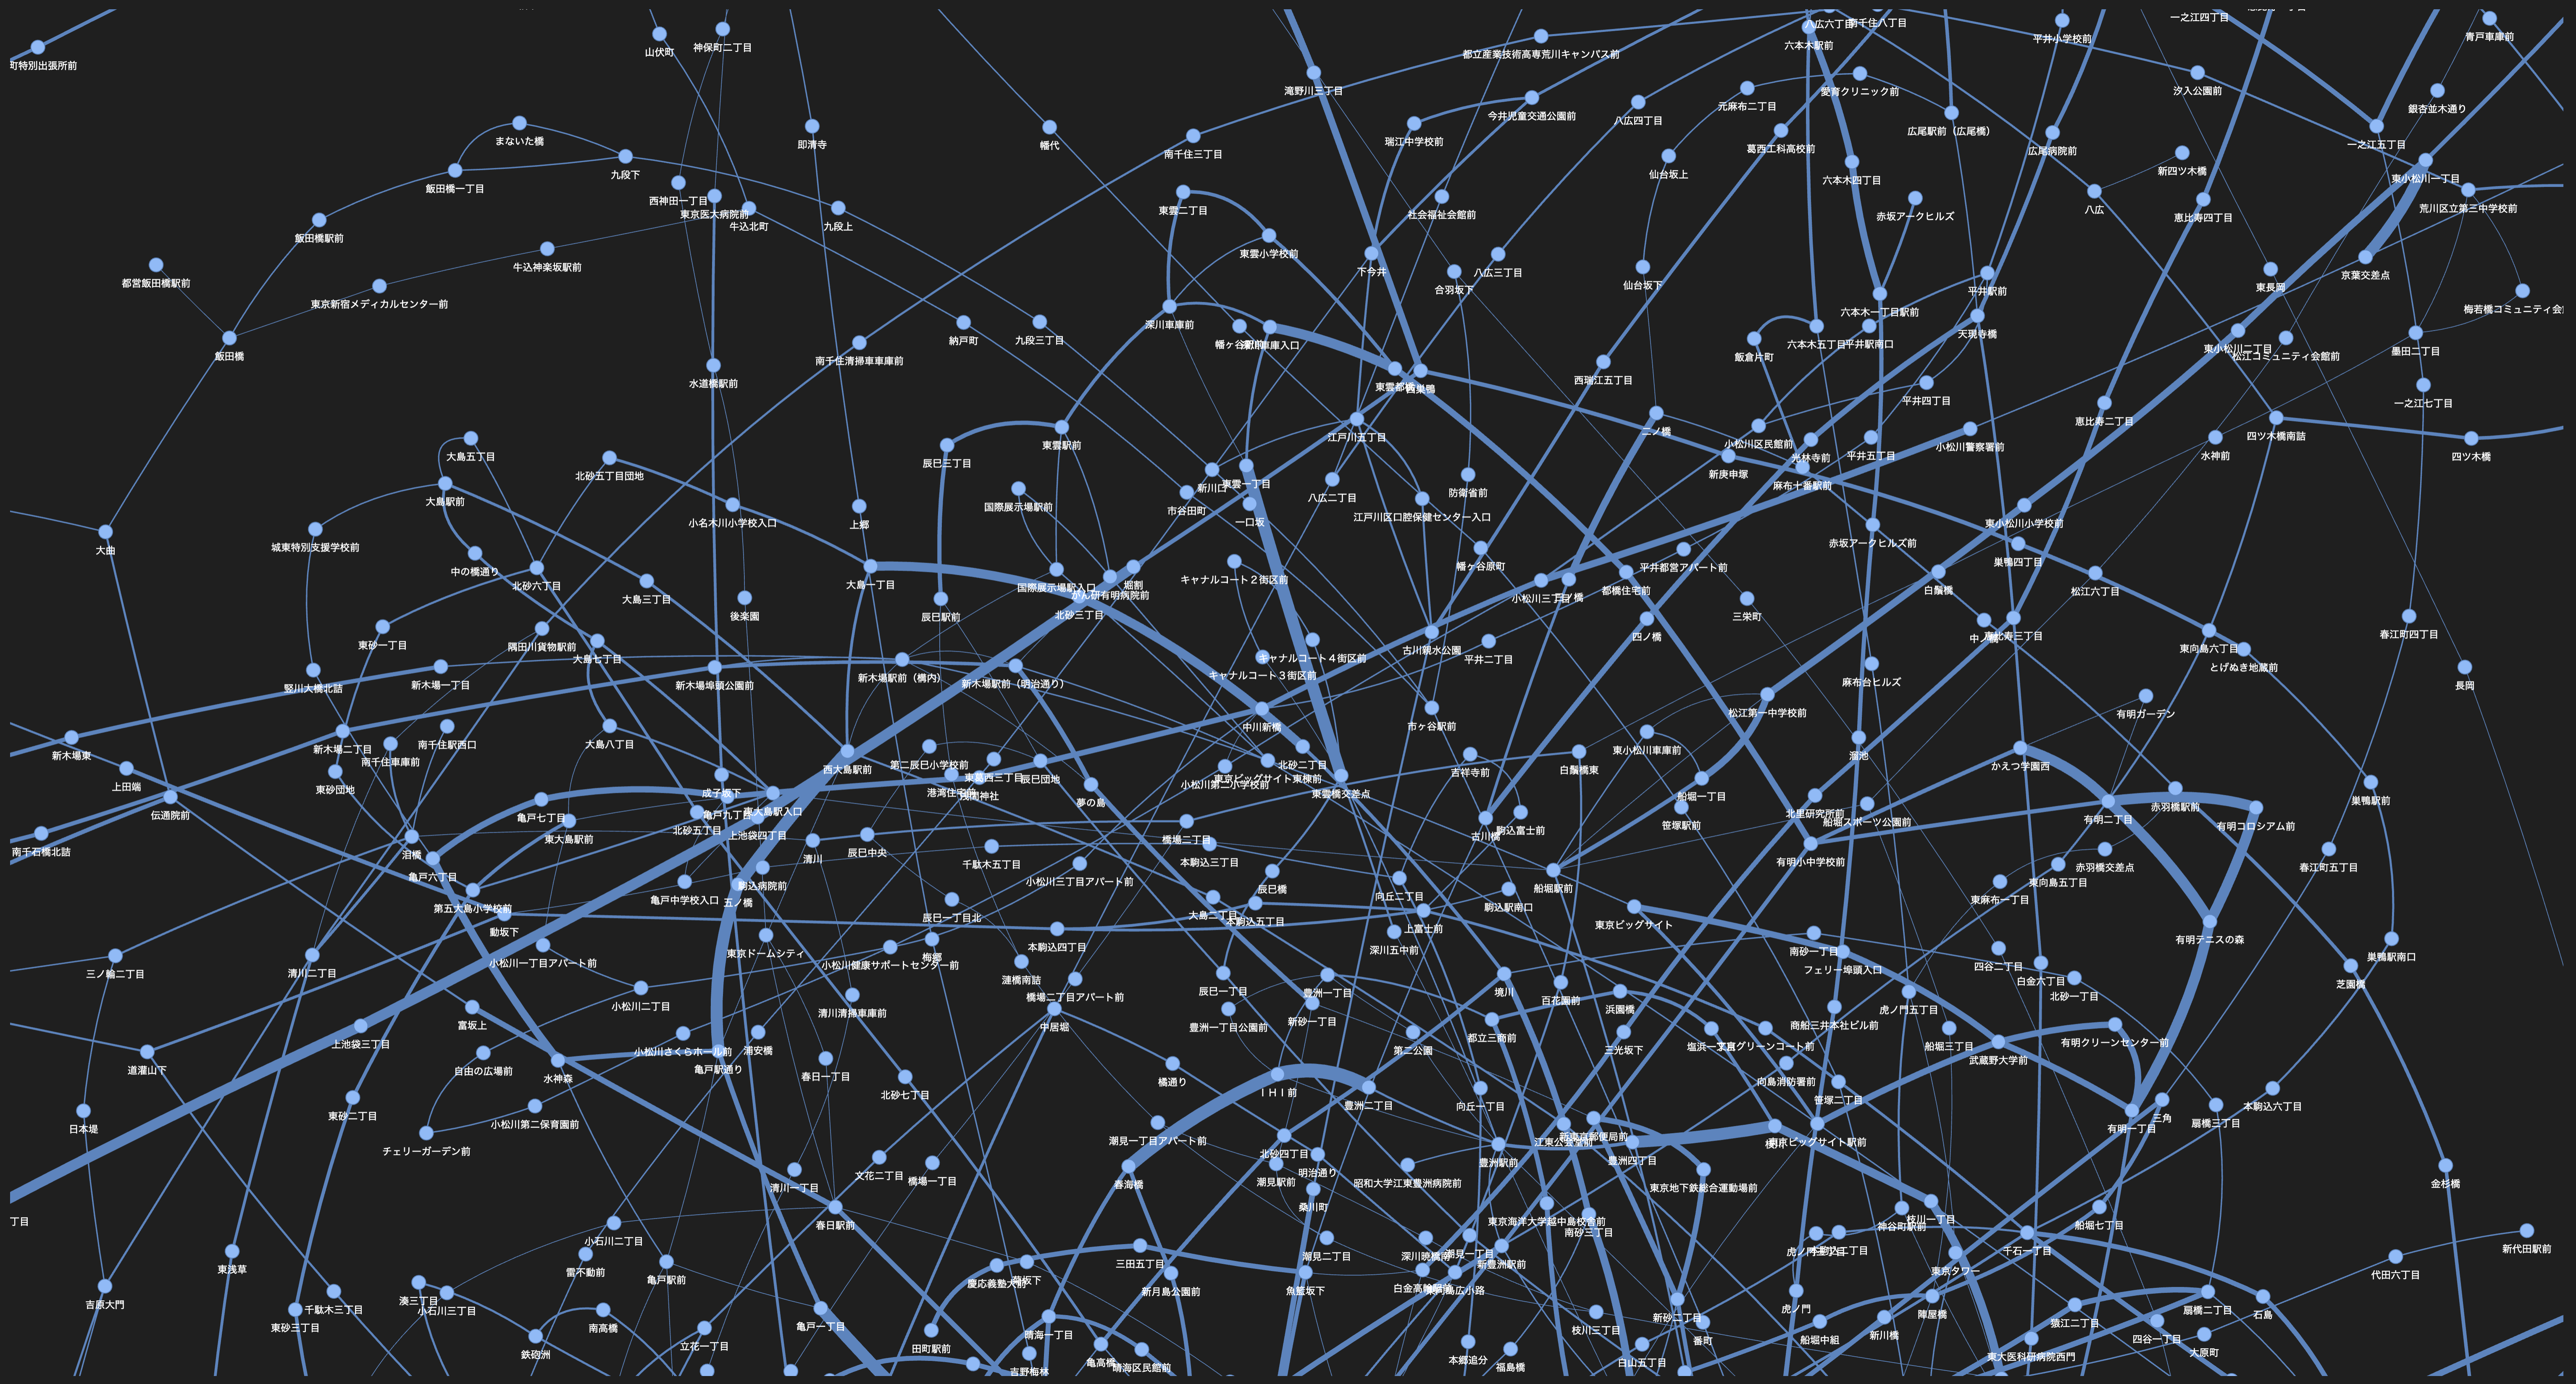
\includegraphics[width=10cm]{./img/fig2.png}
    \caption{可視化表現 ネットワークレイアウト アークグラフ (拡大)}
    \label{fig:fig2}
\end{figure}

\section*{可視化表現の説明}
都営バス\footnote{https://www.kotsu.metro.tokyo.jp/bus/}のGTFS-JP\footnote{https://www.gtfs.jp/}フィード\footnote{https://ckan.odpt.org/dataset/b\_bus\_gtfs\_jp-toei}を用いて,バスの運行状況を可視化する.バス停間の路線数をカウント (同じルートでも別の時間であれば別路線としてカウント) し,ネットワークレイアウトのアークグラフを用いて表した.

Jupyter Notebook\footnote{https://bit.ly/3O5NtKo}上で,Pythonを用いて可視化表現を作成した.

テーブルデータを扱うために,pandasを用いた.

まず,必要なデータフィールドを抽出する.
\begin{figure}[H]
    \centering
    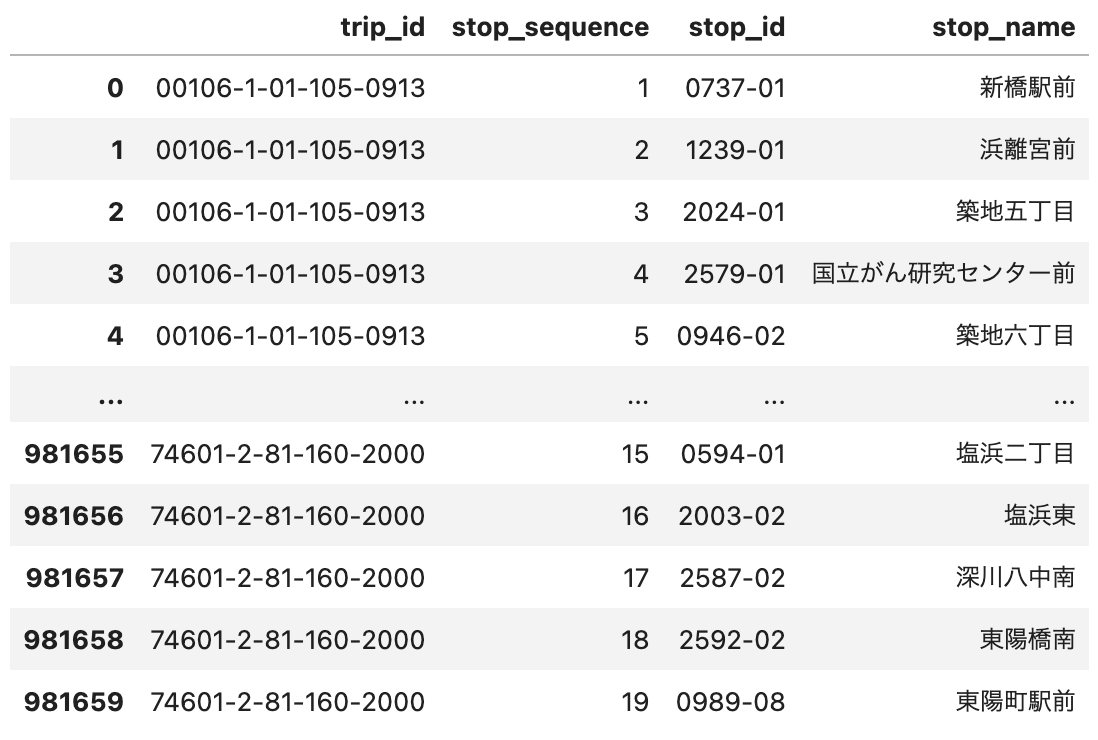
\includegraphics[width=10cm]{./img/table1.png}
    \caption{元データから必要なフィールドを抽出}
    \label{fig:table1}
\end{figure}

次に,バス停間の路線数をカウントする.
\begin{figure}[H]
    \centering
    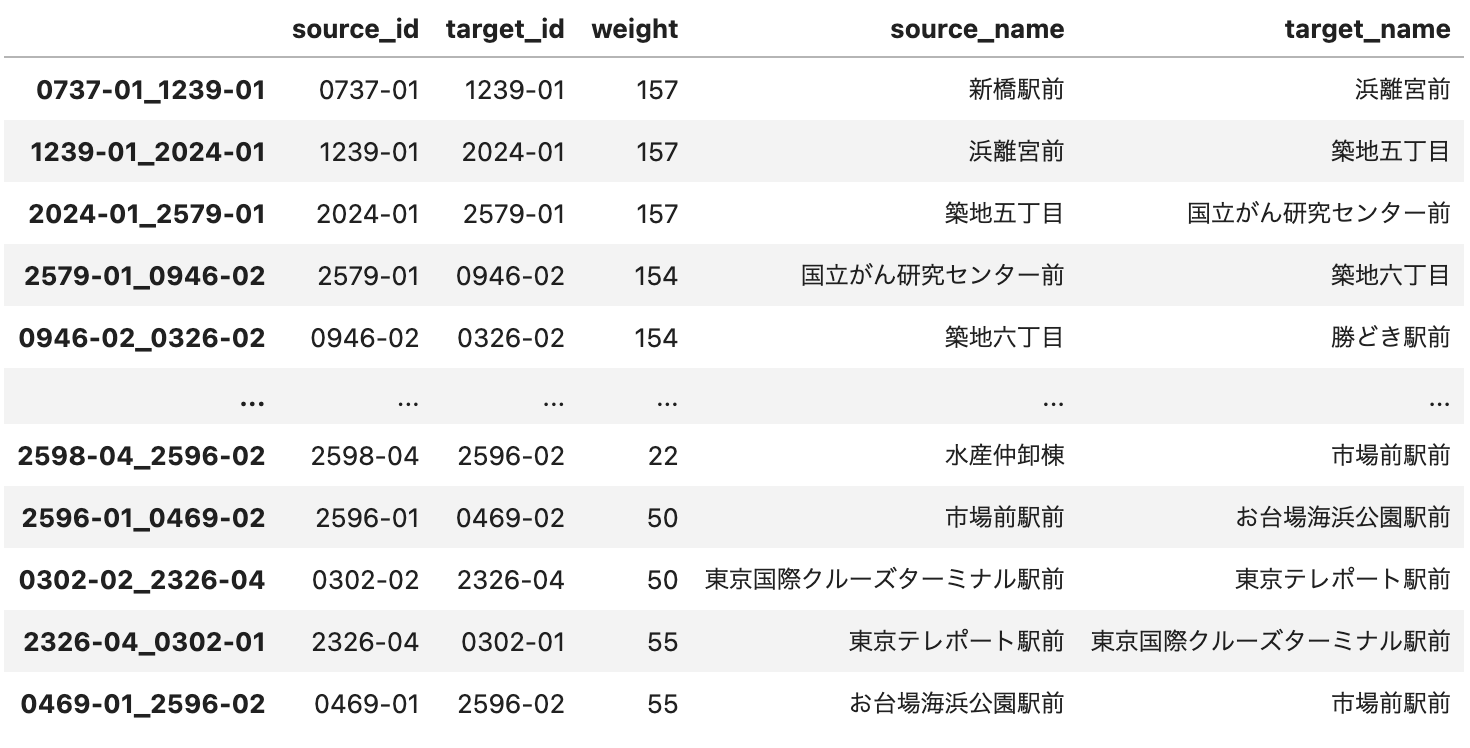
\includegraphics[width=10cm]{./img/table2.png}
    \caption{バス停間の路線数をカウント}
    \label{fig:table2}
\end{figure}

次に,路線数を降順でソートする.
\begin{figure}[H]
    \centering
    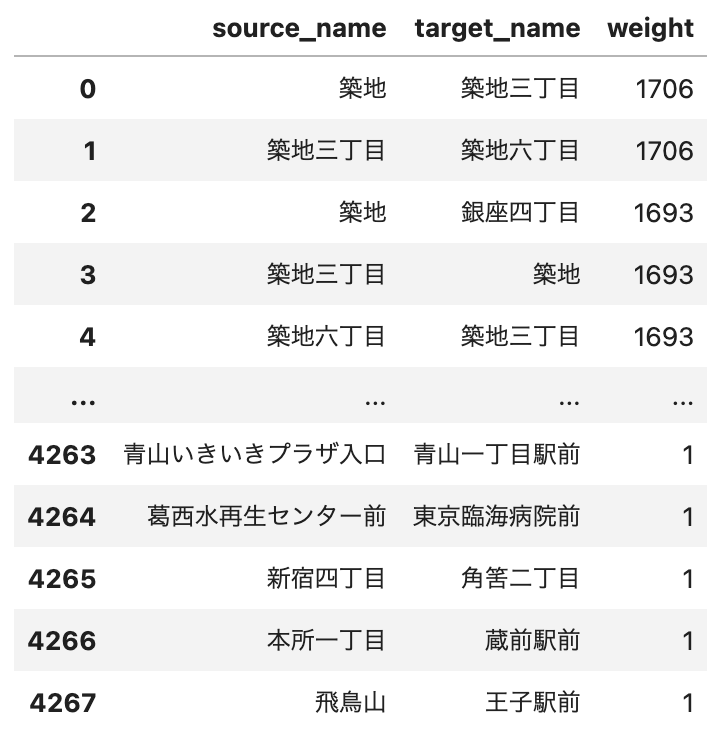
\includegraphics[width=10cm]{./img/table3.png}
    \caption{路線数を降順ソート}
    \label{fig:table3}
\end{figure}

次に,路線数をエッジの太さに対応づけるために,エッジの太さとして適当な範囲の値に調整し,整数型に丸め処理を行う.
\begin{figure}[H]
    \centering
    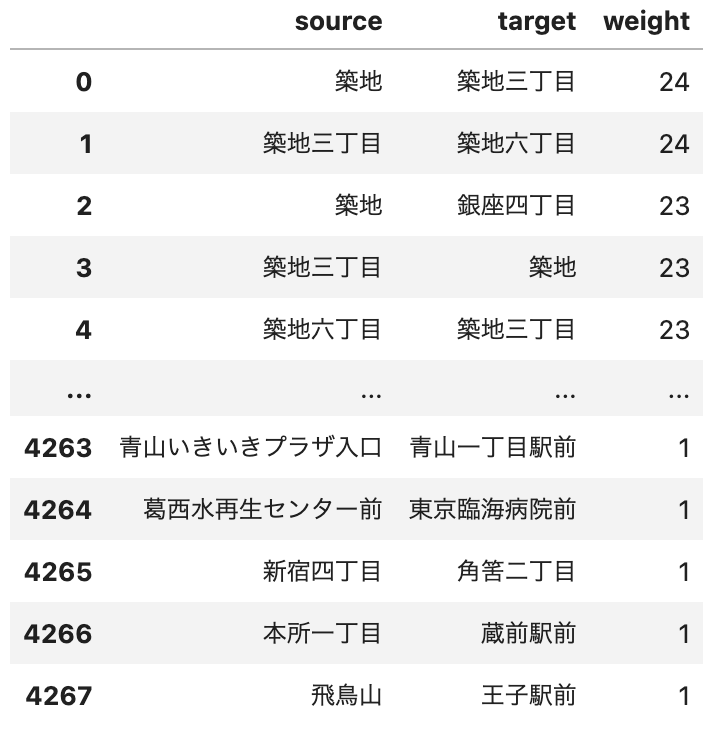
\includegraphics[width=10cm]{./img/table4.png}
    \caption{weightの丸め処理}
    \label{fig:table4}
\end{figure}

このDataFrameと,NetworkX\footnote{https://networkx.org/}のfrom\_pandas\_edgelistメソッド,Pyvis\footnote{https://pyvis.readthedocs.io/en/latest/}のNetworkクラスを用いて,アークグラフを作成した.

\section*{可視化表現からわかること}
可視化表現を見ることで,まず,図\ref{fig:fig1}を見ることで,ノードの数から,バス停数の規模がわかる.他のバス事業者で同じ可視化表現をしたときに,その規模を比べることができる.これは,データファイルのバス停の件数を調べることでもわかる.

また,図\ref{fig:fig1}において,ノードのばらつきやエッジの太さの違いから,バスの路線が多いところがわかる.図\ref{fig:fig2}のように,拡大してみていくと,具体的に,どのバス停の間が特に多いかということが詳細にわかる.そのままだと,エッジが重なり合ってしまい,エッジやノードの位置関係がわかりづらい.そこで,1つのノードを掴んで動かしてみることで,エッジやノードに動きがでる.これにより,エッジやノードの位置関係がより一層わかりやすくなる.これらは,データファイルを眺めるだけでは,わからない.

このグラフの特性から,結びつくバス停の数が多いバス停ほど,真ん中に集まる.そのため,真ん中にあるバス停は,比較的,都市の中心にあるバス停であるのではないかと考えられる.地形によっては,地図上のバス停同士の位置関係とおおよそ一致することがあるかもしれない.

様々な都市のバス事業者のデータを使って,同じ可視化表現を行い,その都市の地図を重ねてみることで,見えてくるのではないかと考えられる.また,同じデータファイルに,座標の情報も含まれるので,それも可視化表現に含めることで,おおよその地図上の位置を保持しつつ,バス停同士の結びつきもわかるような可視化表現が可能になるのではないかと考える.

\end{document}
